\documentclass[border=3pt]{standalone}
% Preâmbulo compartilhado pelos diagramas TikZ da aula 10 (Localização de Markov e Gaussiana)
\usepackage[T1]{fontenc}
\usepackage[utf8]{inputenc}
\usepackage{lmodern}
\usepackage{amsmath}
\usepackage{xcolor}
\usepackage{tikz}
\usetikzlibrary{arrows.meta,angles,quotes,decorations.pathmorphing,calc,
                positioning,shapes.geometric,shapes.misc,backgrounds,fit,
                math}

% Paleta (mesma dos SVGs originais)
\definecolor{dblue}{HTML}{2A5B8C}
\definecolor{dorange}{HTML}{B3541E}
\definecolor{dgreen}{HTML}{4A7C59}
\definecolor{dred}{HTML}{9C4B4B}
\definecolor{dcream}{HTML}{F4F1EA}
\definecolor{dshade}{HTML}{DDD7C9}

% Função gaussiana (não normalizada por padrão de escala visual)
\pgfmathdeclarefunction{gauss}{3}{%
  \pgfmathparse{1/(#3*sqrt(2*pi))*exp(-((#1-#2)^2)/(2*#3^2))}%
}

% Estilos comuns (prefixo d... para não colidir com chaves internas do pgf)
\tikzset{
  >={Stealth[length=2mm]},
  dguide/.style={gray!55, dashed, line width=0.4pt},
  daxis/.style={gray!60, line width=0.7pt, ->},
  dbody/.style={fill=black!3, draw=black!80, line width=1pt},
  dacc/.style={draw=dblue, line width=1pt},
  dlbl/.style={black!55, font=\small},
  dsub/.style={black!45, font=\footnotesize},
  dstate/.style={circle, draw=black!80, fill=dcream, line width=1pt,
                 minimum size=17mm, font=\large, inner sep=1pt},
  dobs/.style={circle, draw=black!80, fill=dshade, line width=1pt,
               minimum size=14mm, font=\large, inner sep=1pt},
  dbox/.style={rounded corners=2pt, draw=black!80, fill=dcream, line width=1pt,
               align=center, inner sep=6pt},
  dop/.style={circle, draw=black!80, fill=white, line width=1pt,
              minimum size=6mm, inner sep=0pt, font=\small},
  dtrans/.style={->, dblue, line width=1pt},
  dmeas/.style={->, dorange, line width=1pt},
  dcurve/.style={line width=1pt, dblue},
  dcurveb/.style={line width=1.4pt, dorange},
}

\usetikzlibrary{shapes.callouts}
\begin{document}
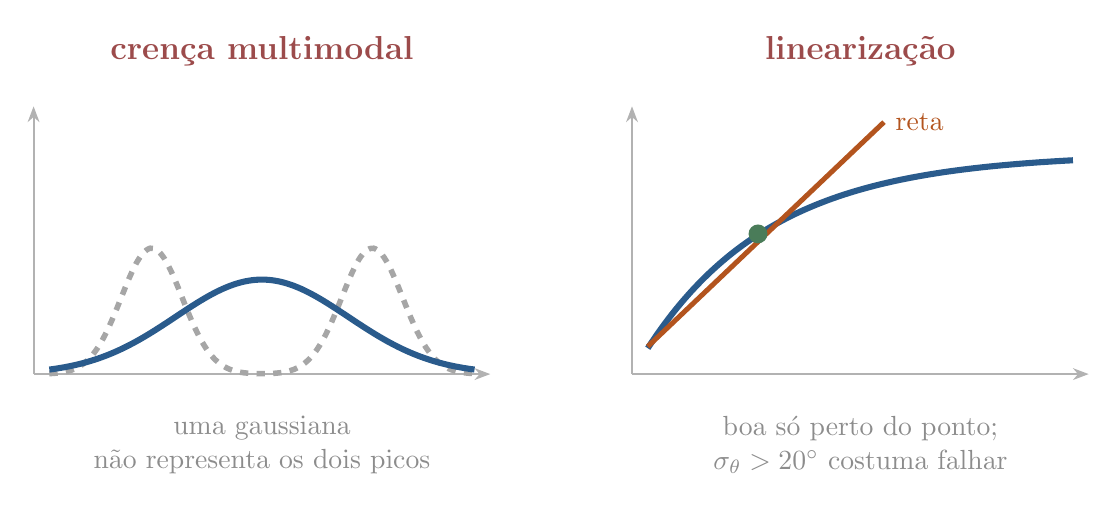
\begin{tikzpicture}[x=1cm,y=1cm,bal/.style={rectangle callout, rounded corners=7pt, draw=black!75, fill=white, line width=1pt, align=center, font=\normalsize, inner sep=5pt}]
\begin{scope}
\draw[daxis] (0,0) -- (5.8,0); \draw[daxis] (0,0) -- (0,3.4);
\draw[black!35, line width=2pt, dashed, domain=0.2:5.6, samples=60, smooth] plot (\x,{1.6*exp(-((\x-1.5)^2)/0.3)+1.6*exp(-((\x-4.3)^2)/0.3)});
\draw[dblue, line width=2.2pt, domain=0.2:5.6, samples=60, smooth] plot (\x,{1.2*exp(-((\x-2.9)^2)/2.4)});
\node[font=\bfseries\large, dred] at (2.9,4.1) {crença multimodal};
\node[dsub, font=\normalsize, align=center] at (2.9,-0.9) {uma gaussiana\\ não representa os dois picos};
\end{scope}
\begin{scope}[shift={(7.6,0)}]
\draw[daxis] (0,0) -- (5.8,0); \draw[daxis] (0,0) -- (0,3.4);
\draw[dblue, line width=2.2pt, domain=0.2:5.6, samples=50, smooth] plot (\x,{2.8*(1-exp(-\x/1.6))});
\draw[dorange, line width=1.8pt] (0.2,0.35) -- (3.2,3.2) node[right, font=\normalsize] {reta};
\fill[dgreen] (1.6,1.78) circle (0.12);
\node[font=\bfseries\large, dred] at (2.9,4.1) {linearização};
\node[dsub, font=\normalsize, align=center] at (2.9,-0.9) {boa só perto do ponto;\\ $\sigma_\theta > 20^\circ$ costuma falhar};
\end{scope}
\end{tikzpicture}
\end{document}
